% SPDX-FileCopyrightText: 2026 Cyprien PIERRE
% SPDX-License-Identifier: CC-BY-4.0
\documentclass[tikz,border=5pt]{standalone}
\usepackage[T1]{fontenc}
\usepackage{lmodern}
\usetikzlibrary{arrows.meta,positioning}
\begin{document}
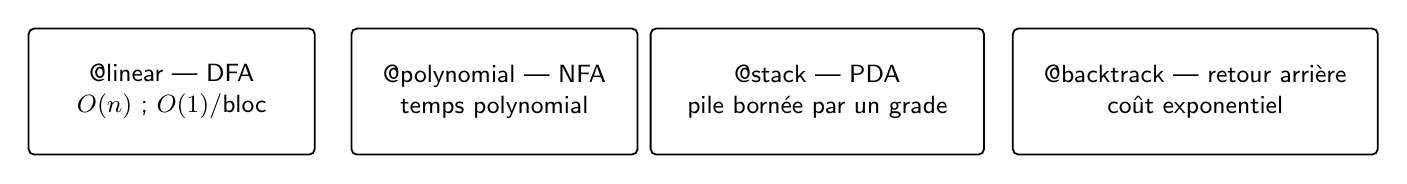
\begin{tikzpicture}[
  font=\sffamily\small,
  box/.style={draw, rounded corners=2pt, align=center, line width=.65pt, minimum height=16mm}
]
\node[box, text width=34mm, minimum width=34mm] (linear) at (18mm,0) {@linear --- DFA\\$O(n)$ ; $O(1)$/bloc};
\node[box, text width=34mm, minimum width=34mm] (poly) at (59mm,0) {@polynomial --- NFA\\temps polynomial};
\node[box, text width=40mm, minimum width=40mm] (stack) at (100mm,0) {@stack --- PDA\\pile bornée par un grade};
\node[box, text width=44mm, minimum width=44mm] (backtrack) at (148mm,0) {@backtrack --- retour arrière\\coût exponentiel};
\end{tikzpicture}
\end{document}
